\section{The fully discrete scheme}%
\label{sec:fully_discrete}
To evolve the system \eqref{eq:ins_semi_discrete} in time, we will for simplicity and ease of explanation use the implicit Backward Euler method. More accurate and efficient methods could be used in the same manner in practice.  For an ordinary differential system of equations of the form
\begin{equation*}
 \Mn \soln_t + \Hn(\soln) = 0
 \, ,
\end{equation*}
where $\soln$ is a function defined on the grid and $\Mn$ is a constant matrix, the backward Euler schemes becomes 
\begin{equation}
  \frac{\Mn (\soln^{i+1} - \soln^i)}{\Delta t} + \Hn(\soln^{i+1}) = 0
  \,.
  \label{eq:backward_euler}
\end{equation}
In~\eqref{eq:backward_euler}, $\Delta t$ is the size of the time step and the superindices $i$ and $i+1$ are the solution at time level $i$ and $i+1$, respectively.

In order to obtain $\soln^{i+1}$, the system of nonlinear equations in~\eqref{eq:backward_euler} must be solved. One strategy is to first form the function in \eqref{eq:intro}, which results in
\begin{equation}
  \Fn(\soln^{i+1}) = 
  \frac{\Mn (\soln^{i+1} - \soln^i)}{\Delta t} + \Hn(\soln^{i+1})
  \,.
  \label{eq:F_function}
\end{equation}
If we find a vector $\soln^*$ such that $\Fn(\soln^*) = 0$, then $\soln^{i+1} = \soln^*$. To solve~\eqref{eq:F_function}, we employ Newton's method~\cite{quarteroni2010numerical}, which is described in \cref{alg:newton}. This allows us to solve a sequence of linear systems of equations and arrive at an approximation of $\soln^{i+1}$.
\begin{algorithm}
\caption{Newton's method}
\label{alg:newton}
\begin{algorithmic}
\STATE{\ \  Input: $\soln^0$ and tolerance $tol$}
\STATE{Output: An approximation of $\soln^*$, where $\Fn(\soln^*) = 0$}
\FOR{$j = 0,1,2, \dots$}
\STATE{solve $J_{\Fn}(\soln^j)\bm{h}^j   = - \Fn(\soln^j)$ \\
set   $\soln^{j+1}  = \soln^j + \bm{h}^j$ \\
\IF{$\|\Fn(\soln^{j+1})\| < tol$} 
		\RETURN  $\soln^{j+1}$
	     \ENDIF}
\ENDFOR
\end{algorithmic}
\end{algorithm}

For the INS equations, $\soln = \wn$, $\Hn(\soln) = \euln(\soln) - \satn(\soln)$, and $\Mn = \Itn$. Hence,~\eqref{eq:F_function} becomes
\begin{equation}
  \Fn(\wn^{i+1}) = 
  \frac{1}{\Delta t} 
  \left(
    \begin{bmatrix}
      \un^{i+1} \\ \vn^{i+1} \\ \zeron
    \end{bmatrix}
    -
    \begin{bmatrix}
      \un^{i} \\ \vn^{i} \\ \zeron
    \end{bmatrix}
    \right)
    + \euln(\wn^{i+1}) - \satn(\wn^{i+1})
  \, . 
  \label{eq:F_function_euler}
\end{equation}
Furthermore, $J_{\Hn}(\wn) = J_{\euln}(\wn) - J_{\satn}(\wn)$, which yields
\begin{equation}
  J_{\Fn}(\wn) =  
  \frac{1}{\Delta t}
  \Itn
  +
  J_{\euln}(\wn)
  -
  J_{\satn}(\wn)
  \, ,
  \label{eq:backward_euler_jacobian}
\end{equation} 
to be used in the Newton iterations. In \eqref{eq:backward_euler_jacobian}, $J_{\euln}(\wn)$ and $J_{\satn}(\wn)$ are given in \Cref{prop:ins} and \Cref{prop:sat}, respectively.

\section{Numerical Experiments}
\label{sec:numerical_experiments}
A simple finite-difference approximation of the Jacobian is given by \cite{knoll2004jacobian} 
\begin{equation}
  J_{i,j} \approx \hat{J}_{i,j} = \frac{\Fn_i(\wn + \delta_j \en_j) - \Fn_i(\wn)}{\delta_j}
  \, .
  \label{eq:J_approx}
\end{equation}
The approximation in \eqref{eq:J_approx} was used during the implementation of the analytical expression of $J_{\Fn}$ since we expected $\|J - \hat{J}\|_{\infty}$ to be small. This allowed us to write unit tests ensuring that the Jacobian has been correctly implemented, by comparing it to the approximation. In \eqref{eq:J_approx}, a small $\delta$ leads to a good approximation. However, note that if $\delta$ is chosen too small, the approximation will be contaminated by floating-point roundoff errors, which limits the practically achievable accuracy of $J$ \cite{knoll2004jacobian}.

Computing difference approximations of the Jacobian also allowed us to compare the efficiency of Newton's method using approximate versus analytical Jacobians. Note that computing the approximation \eqref{eq:J_approx} requires $n$ evaluations of $\Fn$, resulting in $O(n^2)$ complexity, compared to the $O(n)$ complexity of evaluating the exact Jacobian. \Cref{tab:efficiency} shows the execution times for evaluating the analytical Jacobian versus computing the approximation~\eqref{eq:J_approx} at increasing resolutions.

\begin{table}[ht]
  \centering
  \begin{tabular}{|c|c|c|}
    \hline
    Resolution & Exact & FD approximation \\
    \hline
    $5 \times 5$ & 0.005s & 0.858s \\
    $10 \times 10$ & 0.006s & 13.85s \\
    $15 \times 15$ & 0.006s & 76.49s \\
    $20 \times 20$ & 0.007s & 261.6s \\
    \hline
  \end{tabular}
  \caption{Execution times for computing the exact Jacobian of $\Fn$ versus the finite difference approximation~\eqref{eq:J_approx}. Even at low resolutions, using difference approximations of the Jacobian is clearly unrealistic.}
  \label{tab:efficiency}
\end{table}

As expected, due to the large number of evaluations of $\Fn$ needed to compute the approximation, such a strategy quickly becomes infeasible.

It is readily seen that the number of floating point operations needed to evaluate the discrete spatial operator $\euln$ grows linearly with the degrees of freedom $n$. Consider for example the term $\An(I_3 \otimes \Dx)\wn$. The first product, $(I_3 \otimes \Dx) \wn$, are finite difference approximations at each point in the grid, resulting in $Cn$ operations, where $C$ depends on the width of the difference stencil. The matrix $\An$ is a $3$-by-$3$ block matrix with diagonal blocks, and so results in another $O(n)$ number of operations. Analogously, the remaning terms in $\euln$ each contribute $O(n)$ operations. The arithmetic complexity of evaluating a penalty term $\satn$ is $O(\sqrt{n})$ (assuming equal resolution in the horizontal and vertical directions), since $\satn$ acts only on the grid boundary. Hence, the arithmetic complexity of evaluating $\Fn$ is $O(n)$.

Let us study the arithmetic complexity of evaluating the Jacobian $J_{\Fn}$ of $\Fn$. Inspecting the form of the Jacobian $J_{\euln}$ in \Cref{prop:ins} we see a number of terms that need to be evaluated. The partial derivatives $\underline{\Dx \un}$, $\underline{\Dy \vn}$, etc, have already been computed as part of the evaluation of $\euln$, and hence can be disregarded. Similarly, terms that do not depend on the solution, such as $\Dx$, $\Dx^2$, etc, can be disregarded since they remain constant throughout the simulation. Finally we have terms of the type $\Un \Dx$, $\Dy \Vn$, etc. These are all products of a diagonal matrix and a banded difference stencil matrix, and each contribute with $O(n)$ operations. Summing the terms uses $O(n)$ operations. Therefore, the arithmetic complexity of evaluating $J_{\euln}$ is $O(n)$. In fact, the number of operations needed to evaluate products like $\Un \Dx$ or $\Dy \Vn$ do not exceed the number of operations needed to compute the discrete partial derivatives involved in $\euln$. Hence, the cost ratio of evaluating $J_{\euln}$ and evaluating $\euln$ is less than $1$ (i.e. the additional cost of evaluating $J_{\euln}$ is small). As before, the arithmetic complexity of evaluating the Jacobian with respect to a boundary penalty $\satn$ is $O(\sqrt{n})$ since it acts only on the boundary of the grid. Thus, the total arithmetic complexity of evaluating $J_{\Fn}$ is less than the cost of evaluating $\Fn$.


\subsection{The order of accuracy}
The method of manufactured solution \cite{roache2002code} is used to verify the implementation. In all computations in this subsection, the initial guess is the solution from the previous time step and the tolerance $tol$ in \Cref{alg:newton} is set to $10^{-12}$.
For the SBP-operators SBP21 and SBP42, the expected orders of accuracy for the system \eqref{eq:ins_semi_discrete} are 2 and 3, respectively~\cite{svard2006order,svard2019convergence}. The manufactured solution we have used is
\begin{equation}
  \begin{aligned}
    u & = 1 + 0.1 \sin(3\pi x-0.01t)\sin(3\pi y-0.01t)
    \\
    v & = \sin(3\pi x-0.01t)\sin(3\pi y-0.01t)
    \\
    p & = \cos(3\pi x-0.01t)\cos(3\pi y-0.01t)
    \, .
 \end{aligned}
 \label{eq:mms_solution}
\end{equation}
Inserting \eqref{eq:mms_solution} into \eqref{eq:ins_continuous} leads to a non-zero right-hand side $\vecs{k}(t,x,y)$, which is evaluated on the grid and added to the right-hand side of \eqref{eq:ins_semi_discrete} by the vector $\vecs{\kn}(t)$. Since $\vecs{\kn}$ is independent of $\wn$, it does not affect the Jacobian. The initial and boundary data are also taken from \eqref{eq:mms_solution}.
The step size is chosen to be $\Delta t = 10^{-5}$ and the computations are terminated at $t = 1$. Next, we compute the pointwise error vector $\vecs{\en}$ and its $L_2$-norm $\|\vecs{\en}\|_{I_3\otimes \Pn}$. The spatial convergence rate for the SBP operators is given by $r = \log(\|\en\|_{i}/\|\en\|_{j})/\log((j-1)/(i-1))$, where $i$ and $j$ refer to the number of grid points in both spatial dimensions. The order of accuracy in space are presented in \cref{tab:convergence_table} and agree well with theory.
\begin{table}
\centering
\setlength{\tabcolsep}{12pt}
\begin{tabular}{c| cc | cc cc}
 \hline
 \hline
 operator
 & \multicolumn{2}{c|}{SBP21}
 & \multicolumn{2}{c}{SBP42}
 \\
\hline
 \hline
N & $\|\en\|$ & $r$ &$\|\en\|$ & $r$
\\
\hline
21 & 4.13e-02 & --   & 1.90e-02 & -- 
\\   
41 & 9.73e-03 & 2.16 & 2.19e-03 & 3.23
\\
61 & 4.17e-03 & 2.13 & 6.34e-04 & 3.12  
\\
81 & 2.28e-03 & 2.12 & 2.70e-04 & 3.01
\\
\hline
Theoretical && 2 && 3
\end{tabular}
\caption{Error and convergence rate.}%
\label{tab:convergence_table}
\end{table}

Next, we consider the steady-state problem of \eqref{eq:ins_continuous} and \eqref{eq:ins_semi_discrete}, which means that the goal is to find $\wn^*$ such that
\begin{equation}
   \euln(\wn^*) = \satn(\wn^*)
   \, .
   \label{eq:ins_steady_state}
\end{equation}
As before, we want to find an approximation to the vector $\wn^*$ which satisfies
\begin{equation}
  \Fn (\wn^*) = \euln(\wn^*) - \satn(\wn^*) = 0  
  \, .
  \label{eq:F_steady_state}
\end{equation}
The Jacobian of $\Fn$ is $J_{\Fn}(\wn) = J_{\euln}(\wn) - J_{\satn}(\wn)$. 
When the iterate $\wn^k$ is far away from $\wn^*$, Newton's method may not converge and other techniques must initially be applied. We choose the SOR method \cite{quarteroni2010numerical} 
until $\|F(\wn^k)\|_\infty$ is sufficiently small. For SOR, the next iterate is given by $\wn^{k+1} = \wn^k(1-\alpha) + (\wn^k - \hn^k)\alpha$, where $\hn^k$ is the Newton step from \Cref{alg:newton} and $\alpha \in (0,1]$.

To verify our procedure, we choose the steady manufactured solution to be \cite{kovasznay1948laminar} 
\begin{equation}
  \begin{aligned}
    u & = 1-e^{\lambda x} \cos(2\pi y)
    & v & = \frac{1}{2 \pi}\lambda e^{\lambda x}\sin(2\pi y)
    \\
    p & = \frac{1}{2}\left(1 - e^{2\lambda x}\right)
    & \lambda & = \frac{1}{2 \epsilon} - \sqrt{\frac{1}{4 \epsilon^2} + 4 \pi^2}
 \end{aligned}
 \label{eq:mms_solution_steady}
\end{equation}
and the computational domain is changed to $\Omega = [-0.5,1]\times [-1,1]$ for $\epsilon = 1/20$. Inserting \eqref{eq:mms_solution_steady} into the time-independent version of \eqref{eq:ins_continuous} leads to $\vecs{k}(t,x,y) = 0$. The initial guess is $\wn^0 = (1,1, \dots, 1)^\top$ and the tolerance $tol$ in \Cref{alg:newton} is again set to $10^{-12}$. 
%We used $\alpha = 0.5$ until $\|F(\soln^k)\|_\infty < 10^3$. 
\Cref{tab:convergence_table_steady} shows the error and convergence rates, which again agrees well with theory. In \Cref{fig:streamlines}, the streamlines and the velocity field is illustrated for the converged solution on the grid containing $100\times 100$ points. They agree well with previous results \cite{kovasznay1948laminar}. 

\subsection{The convergence rate of the Newton iteration}
Next, we will test the main development in this paper. For $\wn^k$ sufficiently close to $\wn^*$, Newton's method converges quadratically in any norm \cite{quarteroni2010numerical}, which means that $e_{k+1} = C e_k^2$, where $C$ varies marginally between iterations and $e_k = \|\wn^k - \wn^*\|$. To verify that, we consider a grid of size $100\times 100$ with the SBP42 operator. The exact solution $\wn^*$ is approximated by the last iterate. By the assumption that $C$ is constant, the relation

\[
  \frac{e_{k+1}}{e_{k}} \approx
  \left(\frac{e_{k}}{e_{k-1}}\right)^p
\]
is obtained for a general convergence rate $p$, which yields
\[
   p \approx \frac{\log(e_{k+1}/e_k)}{\log(e_{k}/e_{k-1})}
   \, .
\]
The error $e_k = \|\wn^k-\wn^*\|_\infty$ is presented in \Cref{tab:newton_convergence} together with the estimations of $p$. The convergence rate agrees well with the expected theoretical one, which verifies that the Jacobian of $\Fn$ is correct. 
\begin{table}
\centering
\setlength{\tabcolsep}{12pt}
\begin{tabular}{c| cc | cc cc}
 \hline
 \hline
 operator
 & \multicolumn{2}{c|}{SBP21}
 & \multicolumn{2}{c}{SBP42}
 \\
\hline
 \hline
N & $\|\en\|$ & $r$ &$\|\en\|$ & $r$
\\
\hline
21 & 2.04e-01 & --   & 4.95e-02 & --  \\
41 & 4.56e-02 & 2.16 & 6.86e-03 & 2.85 \\
61 & 2.04e-02 & 1.98 & 2.20e-03 & 2.80 \\
81 & 1.16e-02 & 1.97 & 9.76e-04 & 2.83 \\
101& 7.46e-03 & 1.97 & 5.16e-04 & 2.85    
\\
\hline
Theoretical && 2 && 3
\end{tabular}
\caption{Error and (accuracy) convergence rate of \eqref{eq:mms_solution_steady}.}%
\label{tab:convergence_table_steady}
\end{table}

\begin{figure}
 \centering
  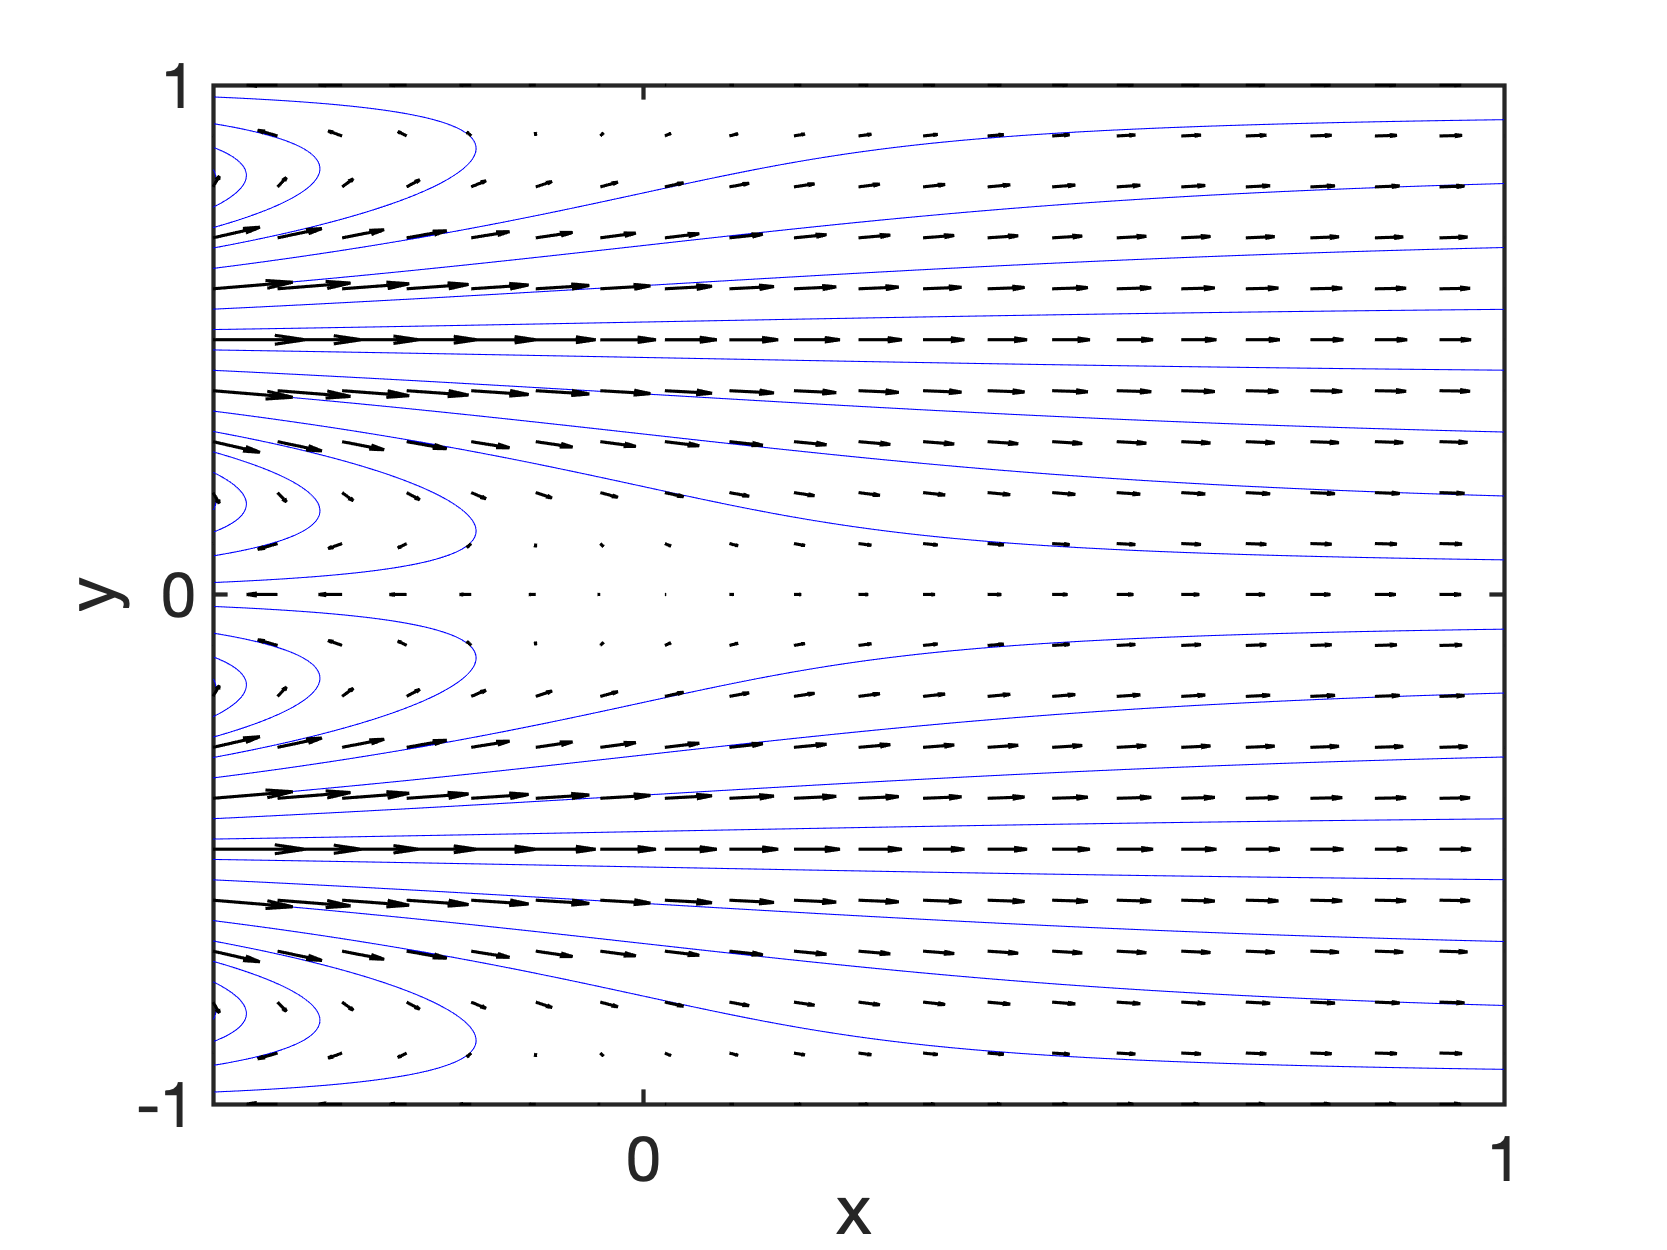
\includegraphics[scale = 0.3]{images/kovaszany}
  \caption{Streamlines and the velocity field of \eqref{eq:mms_solution_steady}.}
  \label{fig:streamlines}
\end{figure}
\begin{table}
\centering
\caption{Errors and the estimated (iterative) convergence rates of \eqref{eq:mms_solution_steady}.}
\begin{tabular}{c| cc }
 \hline
k & $\|e_k\|_\infty$ & $p$
\\
\hline
1 & 3.56e+00  & -- \\
2 & 1.85e+01  & --  \\
3 & 1.89e+00  & -1.38 \\
4 & 1.21e+00  &  0.20 \\
5 & 5.53e-01  &  1.74 \\
6 & 1.10e-01  &  2.07 \\
7 & 3.21e-03  &  2.19 \\
8 & 3.31e-06  &  1.94 \\
9 & 4.14e-12  &  1.98 \\
\hline
Theoretical && 2
\end{tabular}
\label{tab:newton_convergence}
\end{table}

Next, we move on to a more realistic case where the boundary data is set to $g_1 = 1$, $g_2 = g_3 = g_4 = g_5 = g_6 = 0$ and $\epsilon = 0.01$, which will lead to a boundary layer. The computations are performed on $\Omega = [0,1]^2$ with $200\times 200$ grid points with the SBP42 operator. \Cref{fig:boundary_layer} illustrates $\un$ for the converged solution and the iterative convergence order, $p$, is presented in \Cref{tab:boundary_layer}. The estimated iterative convergence order agrees well with what is theoretically expected. 

\begin{figure}
  \centering
  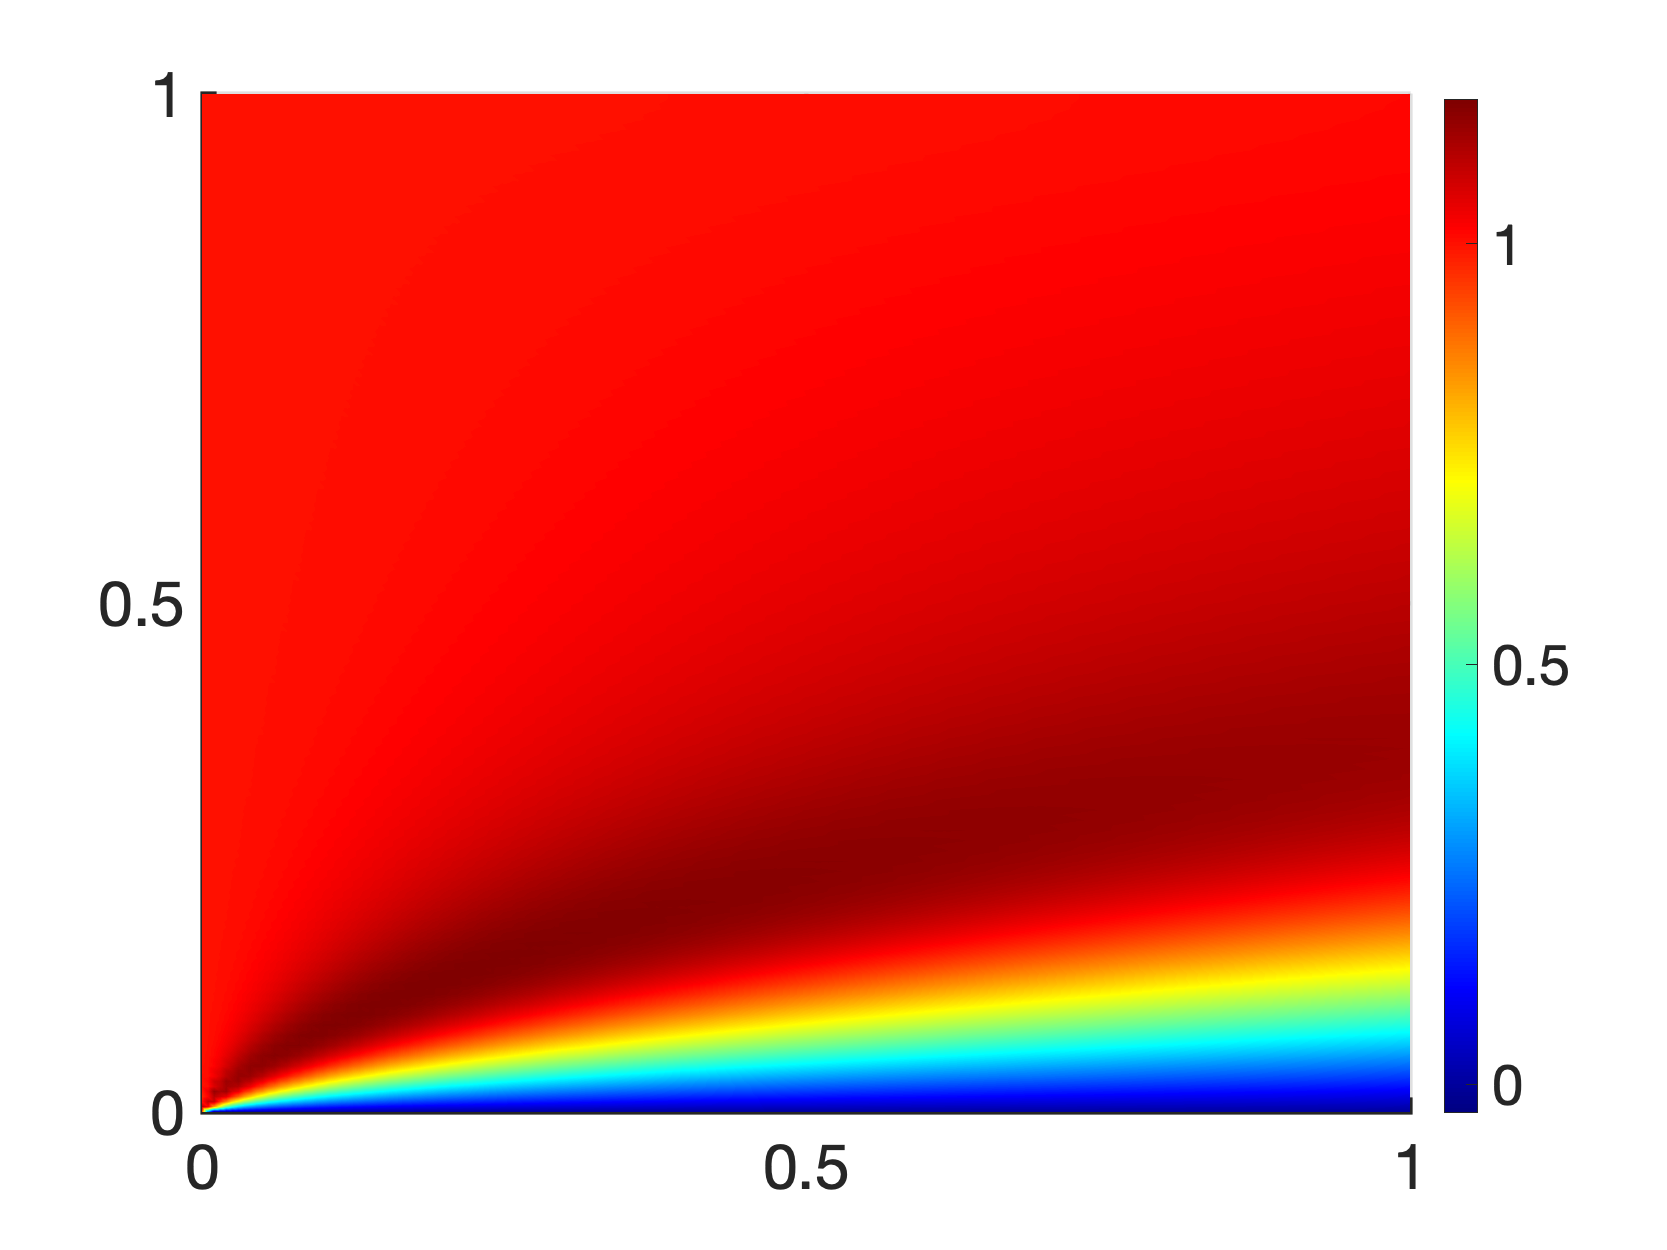
\includegraphics[scale = 0.3]{images/boundary_layer}
  \caption{Flow over a solid surface.}
  \label{fig:boundary_layer}
\end{figure}

\begin{table}
  \centering
  \caption{Errors and the estimated (iterative) convergence rates for the flow over a solid surface.}
  \begin{tabular}{c| cc }
   \hline
  k & $\|e_k\|_\infty$ & $p$
  \\
  \hline
  1 & 1.68e+00  & --  \\
  2 & 6.17e-01  & --  \\
  3 & 1.15e-01  & 1.67 \\
  4 & 4.37e-03  & 1.95 \\
  5 & 1.02e-05  & 1.85 \\
  6 & 5.51e-11  & 2.00 \\
  \hline
  Theoretical && 2
  \end{tabular}
  \label{tab:boundary_layer}
\end{table}

In the last experiment, we consider a curved grid \cite{aalund2019encapsulated} for the incompressible Euler equation (i.e. $\epsilon = 0)$. Both the south and north sides are solid surfaces, where the normal velocity is zero. The west side is an inflow boundary where $u = 1$ and $v = 0$ are specified and at the east side, $p = 0$ is imposed. We change the domain to $\Omega = [-1.5,1.5]\times [0, 0.8]$ and include a smooth bump at the south boundary given by $y(x) = 0.0625e^{-25x^2}$ \cite{bumpgrid} . In \Cref{fig:bump}, the converged solution is illustrated and the estimated iterative convergence rate $p$ is presented in \Cref{tab:bump} for the initial guess $(\un^0;\vn^0;\pn^0) = (1, \dots,1; 0, \dots ,0; 1,\dots 1)$. Again, the results agree well with the theoretical value.
\begin{figure}
 \centering
  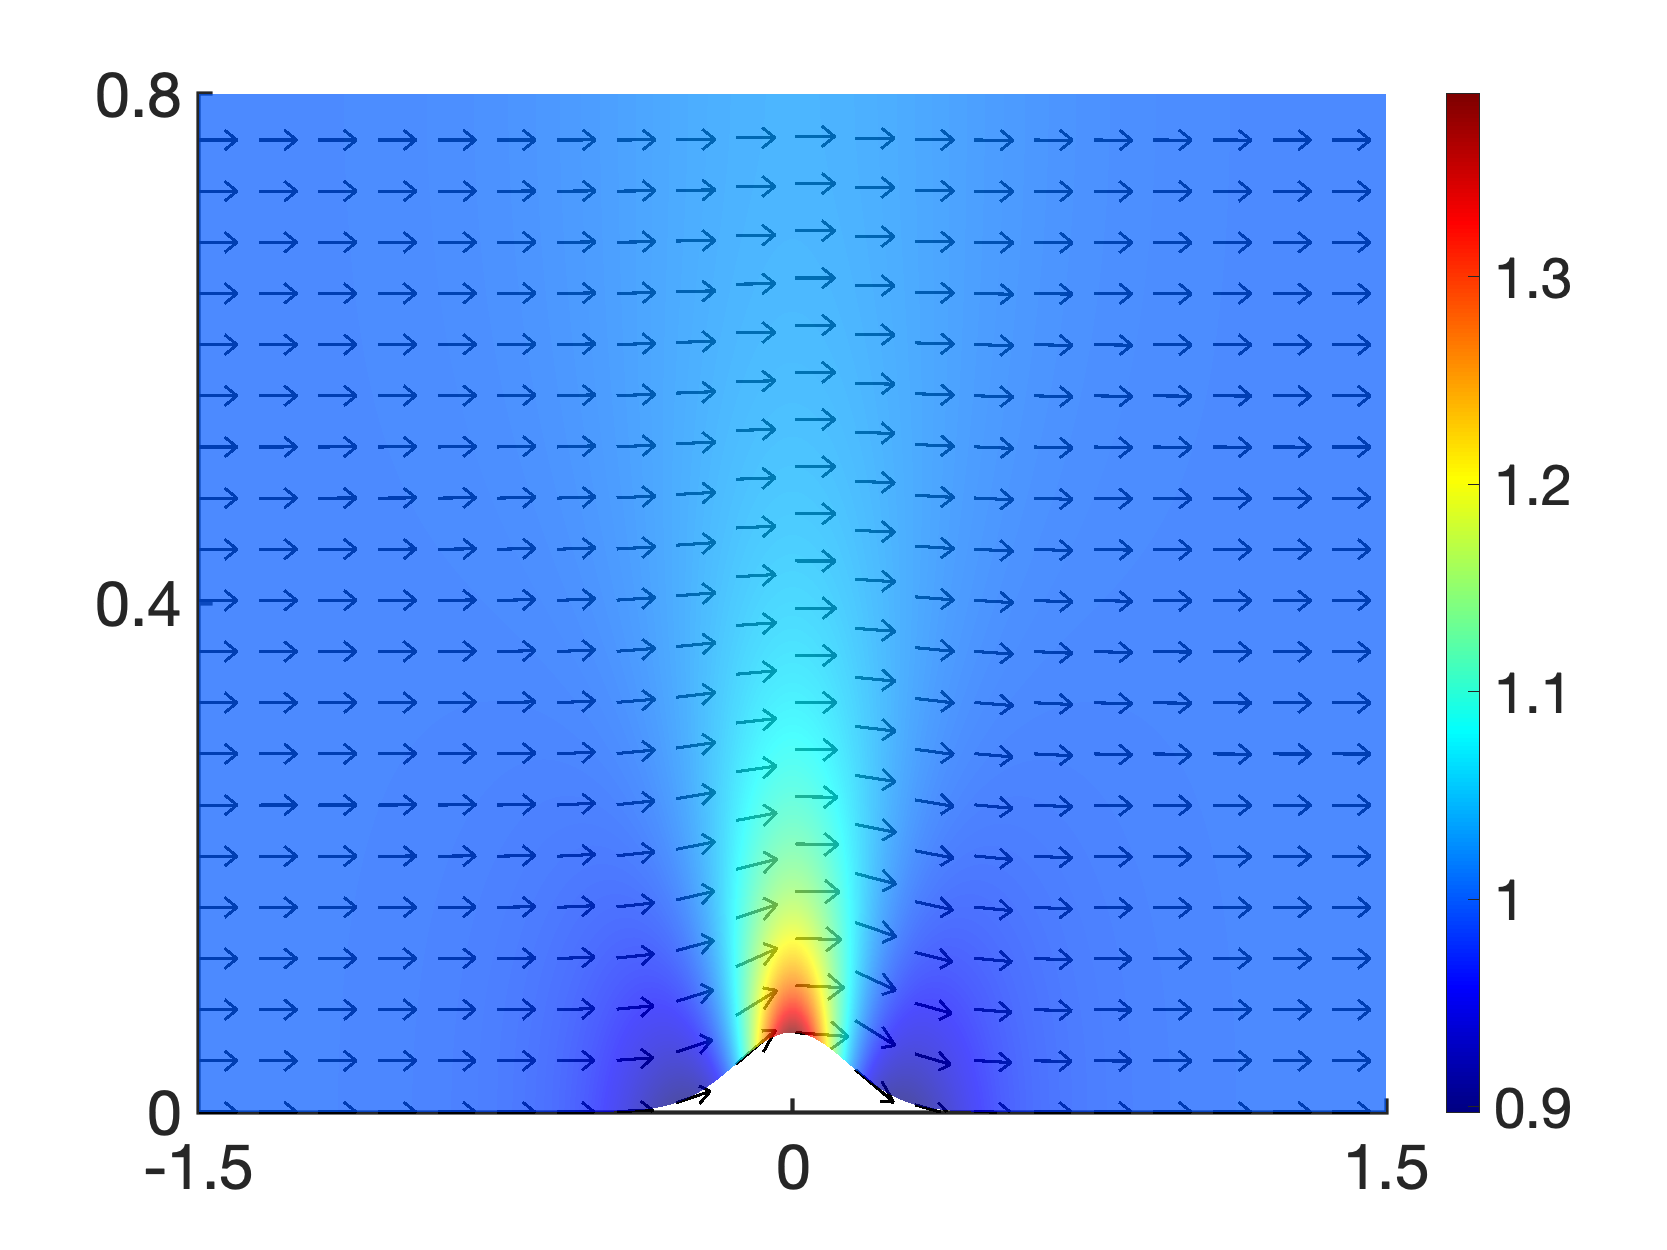
\includegraphics[scale = 0.3]{images/bump.png}
  \caption{Flow over a smooth bump. The plot illustrates the velocity field (arrows) and $\un$ (color figure) at the converged solution.}
  \label{fig:bump}
\end{figure}

\begin{table}
\centering
\caption{Errors and the estimated (iterative) convergence rates for the bump.}
\begin{tabular}{c| cc }
 \hline
k & $\|e_k\|_\infty$ & $p$
\\
\hline
1 &  3.56e+00 & --  \\
2 &  4.91e-01 & --  \\
3 &  1.74e-02 & 1.69 \\
4 &  3.33e-05 & 1.87 \\
5 &  1.55e-10 & 1.96 \\
\hline
Theoretical && 2
\end{tabular}
\label{tab:bump}
\end{table}
